\documentclass[12pt,a4paper]{article}

\usepackage[margin=1in]{geometry}
\usepackage{cite}
\usepackage{amsmath,amssymb,amsfonts}
\usepackage{amsthm}
\newtheorem{proposition}{Proposition}
\usepackage{algorithmic}
\usepackage{algorithm}
\usepackage{graphicx}
\usepackage{textcomp}
\usepackage{xcolor}
\usepackage{hyperref}
\usepackage{booktabs}
\usepackage{multirow}
\usepackage{url}
\usepackage{titlesec}
\usepackage{tikz}
\usepackage{pgfplots}
\usepackage{subcaption}
\usepackage{enumitem}
\usetikzlibrary{arrows.meta,positioning,shapes.geometric,fit,calc}
\pgfplotsset{compat=1.17}

% Section formatting
\titleformat{\section}{\large\bfseries}{\thesection}{1em}{}
\titleformat{\subsection}{\normalsize\bfseries}{\thesubsection}{1em}{}
\titleformat{\subsubsection}{\normalsize\itshape}{\thesubsubsection}{1em}{}

\def\BibTeX{{\rm B\kern-.05em{\sc i\kern-.025em b}\kern-.08em
    T\kern-.1667em\lower.7ex\hbox{E}\kern-.125emX}}

\begin{document}

\title{\textbf{Graph-Structured Adaptive Memory:\\Ontology-Grounded Knowledge Organization\\for Self-Improving Domain Reasoning}}

\author{
Anonymous Authors \\
\textit{Institution Withheld for Review}
}

\date{}

\maketitle

\begin{abstract}
Context adaptation frameworks such as ACE (Agentic Context Engineering) have demonstrated that evolving playbooks of strategies and insights can substantially improve LLM performance on domain-specific tasks. However, these frameworks store accumulated knowledge as flat collections of bullet points, discarding the rich relational structure inherent in specialized domains. In knowledge-intensive fields like financial analysis, domain concepts exist within formal taxonomies (e.g., XBRL hierarchies), formulas depend on entity extraction pipelines, and error patterns cascade through concept dependencies. We introduce \textbf{GSAM} (Graph-Structured Adaptive Memory), a framework that replaces flat bullet storage with an ontology-grounded knowledge graph, where strategies, anti-patterns, domain concepts, and their interrelationships are modeled as typed nodes and edges. GSAM extends the ACE architecture with three contributions: (1) a \textit{Domain Ontology Layer} that anchors learned knowledge to formal taxonomies, enabling principled cross-concept transfer; (2) a \textit{Failure Cascade Model} that represents error propagation chains as first-class graph structures, preventing repeated and downstream failures; and (3) an \textit{Ontology-Aware Retrieval} mechanism that combines graph traversal with embedding similarity, improving retrieval precision by filtering through structural relationships. We evaluate GSAM on financial analysis benchmarks (FiNER and Formula) by extending the ACE codebase, and additionally introduce \textbf{FiNER-Transfer}, a controlled cross-concept transfer benchmark derived from the XBRL taxonomy. Our experimental design targets three hypotheses: that graph structure improves cross-concept transfer, that explicit failure cascades reduce error repetition, and that ontology grounding improves retrieval precision in knowledge-intensive domains.
\end{abstract}

\noindent\textbf{Keywords:} Context Adaptation, Knowledge Graphs, Domain Ontology, Financial Analysis, LLM Memory, XBRL

%==============================================================================
\section{Introduction}
%==============================================================================

Large language model (LLM) applications in specialized domains---such as financial analysis~\cite{loukas2022finer,wang2025finlora}, legal reasoning~\cite{guha2023legalbench}, and biomedical text mining~\cite{lee2020biobert}---demand precise, domain-specific knowledge that goes well beyond what is captured in model weights. Context adaptation~\cite{ace2025}, the practice of modifying LLM inputs with instructions, strategies, and domain evidence rather than updating weights, has emerged as a practical paradigm for closing this gap. It offers interpretability~\cite{wei2022chain}, rapid integration of new knowledge~\cite{lewis2020retrieval}, and shareability across models~\cite{khot2022decomposed}.

Recent frameworks have made important progress. Dynamic Cheatsheet (DC)~\cite{suzgun2025dynamic} introduced test-time memory that accumulates strategies across tasks. ACE (Agentic Context Engineering)~\cite{ace2025} addressed two critical failure modes---\textit{brevity bias} (where optimization collapses toward short summaries that lose domain detail) and \textit{context collapse} (where iterative LLM rewrites degrade accumulated knowledge)---through a multi-agent architecture (Generator, Reflector, Curator) with incremental delta updates. On financial benchmarks, ACE demonstrated average gains of 8.6\% over strong baselines~\cite{ace2025}.

Yet both DC and ACE store accumulated knowledge as \textit{flat collections of bullet points}. Each bullet is an independent unit with metadata (helpful/harmful counters) but no explicit connections to other bullets. This design discards a critical signal: the \textit{relationships between knowledge elements}. In knowledge-intensive domains, these relationships are not merely useful---they are the primary organizing principle of the domain itself. Consider three concrete limitations:

\paragraph{(L1) No Cross-Concept Transfer.} Financial entity recognition involves 139 fine-grained XBRL entity types~\cite{loukas2022finer} organized in a formal taxonomy. A strategy that helps distinguish \texttt{Revenue} from \texttt{OtherIncome} likely transfers to distinguishing \texttt{OperatingExpenses} from \texttt{NonOperatingExpenses}---not because the surface descriptions are similar, but because both require the same structural reasoning about XBRL hierarchies. Flat bullet storage, which relies on embedding similarity between task descriptions, cannot capture this.

\paragraph{(L2) No Failure Propagation Modeling.} In the Formula benchmark~\cite{wang2025finlora}, numerical reasoning depends on correct entity extraction. If the model learns that ``confusing \texttt{NetIncome} with \texttt{ComprehensiveIncome}'' is a failure pattern, this knowledge should propagate to every formula that uses either entity. In flat storage, the anti-pattern bullet is isolated---it has no links to the formulas it affects.

\paragraph{(L3) Retrieval by Similarity, Not Relevance.} When the Generator faces a new question about \texttt{EarningsPerShare}, flat retrieval surfaces bullets whose text is embedding-similar to ``earnings per share.'' But the most relevant knowledge might be a strategy about extracting \texttt{WeightedAverageShares} (a dependency of EPS) or an anti-pattern about confusing basic vs.\ diluted shares---items that are \textit{structurally} relevant but not necessarily \textit{textually} similar.

We introduce \textbf{GSAM} (Graph-Structured Adaptive Memory), a framework that replaces flat bullet storage with an ontology-grounded knowledge graph, where domain concepts, strategies, anti-patterns, and their interrelationships are modeled as typed nodes and edges. GSAM extends the ACE architecture with three contributions:

\begin{enumerate}[leftmargin=*]
\item \textbf{Domain Ontology Layer (\S\ref{sec:ontology}).} GSAM anchors learned knowledge to formal domain taxonomies (e.g., XBRL hierarchies for finance). This provides a structural backbone for cross-concept transfer: knowledge about one part of the taxonomy can propagate to structurally similar regions.

\item \textbf{Failure Cascade Model (\S\ref{sec:failure}).} Anti-patterns are modeled as first-class graph nodes with explicit edges to the concepts, formulas, and strategies they affect. This enables reasoning about error propagation: ``If entity X is misidentified, formulas Y and Z that depend on X are also at risk.''

\item \textbf{Ontology-Aware Retrieval (\S\ref{sec:retrieval}).} Retrieval combines embedding similarity with graph traversal, first identifying relevant concept nodes, then walking dependency and taxonomic edges to surface structurally related strategies and anti-patterns.
\end{enumerate}

We evaluate GSAM by extending the ACE codebase on two financial analysis benchmarks---FiNER~\cite{loukas2022finer} (139-type entity recognition) and Formula~\cite{wang2025finlora} (numerical reasoning over XBRL filings)---and introduce \textbf{FiNER-Transfer}, a controlled benchmark for measuring cross-concept transfer within the XBRL taxonomy. Our experimental design tests three hypotheses:

\begin{itemize}[leftmargin=*]
\item[\textbf{H1}] Graph-structured memory with ontology grounding improves cross-concept transfer compared to flat storage.
\item[\textbf{H2}] Explicit failure cascade modeling reduces repeated and downstream errors.
\item[\textbf{H3}] Ontology-aware retrieval achieves higher precision than embedding-only retrieval.
\end{itemize}

We focus exclusively on domain-specific knowledge tasks rather than agent benchmarks (e.g., AppWorld) for two reasons. First, domain-specific tasks have inherent relational structure (taxonomies, formula dependencies) that provides a clear test bed for graph-structured memory. Second, this focus allows controlled experiments that isolate the effect of knowledge representation from the confounding factors of agent execution (tool use, environment interaction, code generation).

%==============================================================================
\section{Background and Motivation}
\label{sec:background}
%==============================================================================

\subsection{Context Adaptation}

Context adaptation (or context engineering) improves model behavior by constructing or modifying inputs to an LLM rather than altering its weights~\cite{ace2025}. The paradigm has evolved from simple in-context learning with demonstrations~\cite{brown2020language,agarwal2024manyshot} to sophisticated feedback-driven systems: Reflexion~\cite{shinn2023reflexion} reflects on agent failures, TextGrad~\cite{yuksekgonul2024textgrad} optimizes prompts via gradient-like textual feedback, and GEPA~\cite{agrawal2025gepa} uses genetic Pareto search over prompt variants.

Two recent systems are most relevant to our work. Dynamic Cheatsheet~\cite{suzgun2025dynamic} introduces an external memory of reusable strategies accumulated during test-time inference. ACE~\cite{ace2025} builds on this with three innovations: (1) a dedicated Reflector that separates insight extraction from curation, (2) incremental delta updates that prevent context collapse, and (3) a grow-and-refine mechanism that balances context expansion with redundancy control. ACE achieves state-of-the-art results on both agent and domain-specific benchmarks.

\subsection{The Flat Storage Bottleneck}
\label{sec:flat-bottleneck}

Both DC and ACE represent accumulated knowledge as ordered lists of bullets:
\begin{equation}
\mathcal{B} = \{b_1, b_2, \ldots, b_M\}, \quad b_j = (\text{id}_j,\ \text{content}_j,\ h_j,\ n_j)
\label{eq:bullets}
\end{equation}
where $h_j$ and $n_j$ count how often bullet $b_j$ was marked helpful or harmful. Retrieval for a new query $q$ selects bullets by embedding cosine similarity: $\text{retrieve}(q) = \text{top-}k_{b \in \mathcal{B}} \cos(\phi(q), \phi(b))$.

This design has three structural properties that become limitations in knowledge-intensive domains:

\textbf{Independence Assumption.} Each bullet is treated as an independent unit. There is no mechanism to express that bullet $b_i$ (a strategy) depends on bullet $b_j$ (an API usage pattern), or that bullet $b_k$ (an anti-pattern) is the failure mode of $b_i$.

\textbf{Flat Namespace.} All bullets share a single semantic space for retrieval. Domain concepts, strategies, troubleshooting tips, and code snippets compete for the same $k$ retrieval slots, leading to heterogeneous and potentially noisy context windows.

\textbf{No Structural Priors.} The system has no way to incorporate known domain structure. In finance, the XBRL taxonomy defines a hierarchy of 139+ entity types. In medicine, ICD codes form a tree. These structures could guide both knowledge organization and retrieval, but flat storage cannot leverage them.

\subsection{Why Financial Analysis Is the Right Test Bed}

We focus on financial analysis for three specific reasons that make it an ideal domain for evaluating graph-structured memory:

\textbf{Formal Ontology.} XBRL (eXtensible Business Reporting Language) defines a formal taxonomy of financial concepts with explicit hierarchical relationships (e.g., \texttt{Assets} $\rightarrow$ \texttt{CurrentAssets} $\rightarrow$ \texttt{CashAndCashEquivalents}). This provides ground-truth structure against which we can evaluate whether our graph captures meaningful relationships.

\textbf{Cross-Task Dependencies.} FiNER (entity recognition) and Formula (numerical reasoning) operate on the same underlying concepts: a formula like $\texttt{EPS} = \texttt{NetIncome} / \texttt{WeightedAverageShares}$ depends on correctly extracting both entities. This creates a natural cross-task dependency graph.

\textbf{Compositional Error Structure.} Financial reasoning errors often cascade: misidentifying an entity leads to incorrect formula inputs, which produces wrong numerical answers. This cascade structure is naturally captured by graphs but invisible in flat storage.

\subsection{Knowledge Graphs for Domain Knowledge}

Knowledge graphs (KGs) represent structured information as typed entities and relations~\cite{hogan2021knowledge}. They have been applied to question answering~\cite{yasunaga2021qagnn}, commonsense reasoning~\cite{wang2021logic}, and biomedical discovery~\cite{zhu2023llms}. Recent work has explored KGs for LLM augmentation: KAPING~\cite{baek2023kaping} retrieves KG subgraphs to augment prompts, and KG-Agent~\cite{jiang2024kgagent} uses KGs to guide multi-step reasoning.

Our work differs from these in a critical way: rather than using a \textit{pre-existing} KG to augment LLM inputs, we \textit{construct} a KG dynamically from the LLM's own learning process, grounding it in a domain ontology. The graph evolves as the system encounters new tasks, making it a \textit{living memory} rather than a static knowledge base.

%==============================================================================
\section{Problem Formulation}
\label{sec:formulation}
%==============================================================================

Let $\mathcal{T} = \{t_1, \ldots, t_N\}$ be a sequence of domain-specific tasks. Each task $t_i = (c_i, q_i, y_i)$ consists of a context $c_i$ (e.g., a financial document excerpt), a question $q_i$, and a ground-truth answer $y_i$. The system produces a prediction $\hat{y}_i$ and receives feedback $f_i$ (correct/incorrect, with optional reasoning trace).

\textbf{Flat Storage (ACE Baseline).} As in Eq.~\ref{eq:bullets}, knowledge is a set $\mathcal{B}$ of independent bullets. After each task, the Reflector extracts insights and the Curator produces delta bullets $\Delta\mathcal{B}_i$, which are merged: $\mathcal{B} \leftarrow \mathcal{B} \cup \Delta\mathcal{B}_i$.

\textbf{Graph-Structured Memory (GSAM).} Knowledge is a typed, attributed graph $G = (V, E, \tau_V, \tau_E, \alpha)$ where:

\begin{itemize}[leftmargin=*]
\item $V$ is a set of nodes, each assigned a type $\tau_V(v) \in \{\textsc{Strategy}, \textsc{AntiPattern}, \textsc{Concept}, \textsc{Formula}, \textsc{Confusion}\}$.
\item $E \subseteq V \times V$ is a set of directed edges, each assigned a type $\tau_E(e) \in \mathcal{R}$.
\item $\alpha: V \cup E \rightarrow \mathcal{A}$ maps nodes and edges to attribute dictionaries (natural language content, counters, confidence scores).
\end{itemize}

The relation set $\mathcal{R}$ encodes domain-specific semantics:

\begin{equation}
\mathcal{R} = \left\{
\begin{array}{l}
\texttt{is\_a},\ \texttt{part\_of},\ \texttt{depends\_on},\ \texttt{applies\_to},\\
\texttt{fails\_for},\ \texttt{fixes},\ \texttt{confused\_with},\ \texttt{conflicts\_with}
\end{array}
\right\}
\label{eq:relations}
\end{equation}

Given a new task $t_i$, GSAM retrieves a relevant subgraph $G_i \subseteq G$ and serializes it into a structured context that is provided to the Generator alongside the task.

%==============================================================================
\section{Methodology}
\label{sec:method}
%==============================================================================

GSAM extends the ACE architecture by replacing the flat bullet store with a graph-structured memory module. We retain ACE's Generator, Reflector, and Curator roles, and add two new components: the \textbf{Graph Constructor} (which builds and maintains the knowledge graph) and the \textbf{Graph Retriever} (which extracts relevant subgraphs for new tasks). Figure~\ref{fig:architecture} illustrates the full architecture.

\begin{figure}[t]
\centering
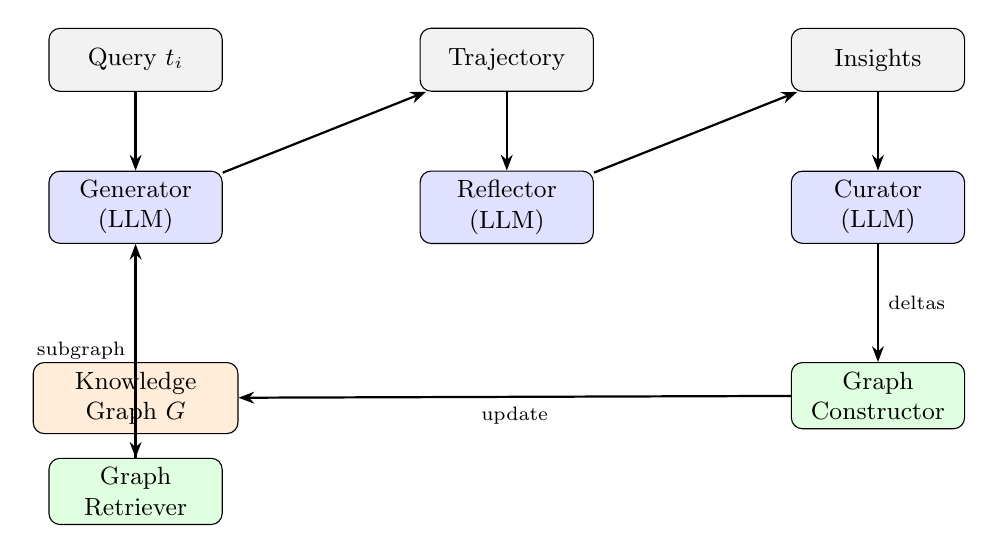
\begin{tikzpicture}[
    node distance=1.2cm and 1.8cm,
    box/.style={rectangle, draw, rounded corners, minimum width=2.2cm, minimum height=0.8cm, font=\small, align=center},
    agent/.style={box, fill=blue!12},
    store/.style={box, fill=orange!15, minimum width=2.6cm},
    arrow/.style={-{Stealth[length=2mm]}, thick},
    label/.style={font=\scriptsize, midway}
]
% Nodes
\node[agent] (gen) {Generator\\(LLM)};
\node[agent, right=2.5cm of gen] (ref) {Reflector\\(LLM)};
\node[agent, right=2.5cm of ref] (cur) {Curator\\(LLM)};
\node[box, fill=green!12, below=1.5cm of cur] (gc) {Graph\\Constructor};
\node[store, below=1.5cm of gen] (kg) {Knowledge\\Graph $G$};
\node[box, fill=green!12, below=0.3cm of kg] (gr) {Graph\\Retriever};
\node[box, fill=gray!10, above=1cm of gen] (query) {Query $t_i$};
\node[box, fill=gray!10, above=1cm of ref] (traj) {Trajectory};
\node[box, fill=gray!10, above=1cm of cur] (insights) {Insights};

% Arrows
\draw[arrow] (query) -- (gen);
\draw[arrow] (gen) -- (traj) node[label, above] {};
\draw[arrow] (traj) -- (ref);
\draw[arrow] (ref) -- (insights) node[label, above] {};
\draw[arrow] (insights) -- (cur);
\draw[arrow] (cur) -- (gc) node[label, right] {deltas};
\draw[arrow] (gc) -- (kg) node[label, below] {update};
\draw[arrow] (gr) -- (gen) node[label, left] {subgraph};
\draw[arrow, dashed] (kg) -- (gr);

\end{tikzpicture}
\caption{\textbf{GSAM Architecture.} The Generator, Reflector, and Curator are inherited from ACE. GSAM adds a Graph Constructor (which converts Curator deltas into graph operations) and a Graph Retriever (which extracts relevant subgraphs for each new query). The Knowledge Graph $G$ replaces ACE's flat bullet store.}
\label{fig:architecture}
\end{figure}


\subsection{Knowledge Graph Schema}
\label{sec:schema}

Table~\ref{tab:schema} defines the node and edge types in the GSAM schema for financial analysis.

\begin{table}[t]
\centering
\caption{GSAM Knowledge Graph Schema for Financial Analysis}
\label{tab:schema}
\small
\begin{tabular}{@{}llp{6.5cm}@{}}
\toprule
\textbf{Component} & \textbf{Type} & \textbf{Description and Attributes} \\
\midrule
\multicolumn{3}{l}{\textit{Node Types}} \\
\midrule
\textsc{Strategy} & Node & Reusable approach or pattern. Attrs: content, helpful count, harmful count, confidence. \\
\textsc{AntiPattern} & Node & Failed approach to avoid. Attrs: content, failure count, root cause, severity. \\
\textsc{Concept} & Node & Domain concept (e.g., XBRL entity type). Attrs: name, definition, taxonomy path. \\
\textsc{Formula} & Node & Computational rule. Attrs: expression, input entities, output entity. \\
\textsc{Confusion} & Node & Documented confusion between entities. Attrs: entity pair, distinguishing criteria. \\
\midrule
\multicolumn{3}{l}{\textit{Edge Types}} \\
\midrule
\texttt{is\_a} & Edge & Taxonomic: child $\rightarrow$ parent in XBRL hierarchy. \\
\texttt{part\_of} & Edge & Compositional: component $\rightarrow$ aggregate. \\
\texttt{depends\_on} & Edge & Computational: formula $\rightarrow$ required entity. \\
\texttt{applies\_to} & Edge & Strategy $\rightarrow$ Concept it addresses. \\
\texttt{fails\_for} & Edge & AntiPattern $\rightarrow$ Concept where it fails. \\
\texttt{fixes} & Edge & Strategy $\rightarrow$ AntiPattern it resolves. \\
\texttt{confused\_with} & Edge & Concept $\leftrightarrow$ Concept (bidirectional). \\
\texttt{conflicts\_with} & Edge & Strategy $\leftrightarrow$ Strategy (mutually exclusive). \\
\bottomrule
\end{tabular}
\end{table}

The schema distinguishes between \textit{domain-structural} edges (\texttt{is\_a}, \texttt{part\_of}, \texttt{depends\_on}) that encode the formal ontology, and \textit{experiential} edges (\texttt{applies\_to}, \texttt{fails\_for}, \texttt{fixes}, \texttt{confused\_with}) that are learned from execution feedback. This separation is a key design choice: domain-structural edges can be initialized from the ontology before any tasks are executed, while experiential edges accumulate during adaptation.


\subsection{Domain Ontology Layer}
\label{sec:ontology}

A distinguishing feature of GSAM is its use of a formal domain ontology as a structural backbone for the knowledge graph.

\textbf{Ontology Initialization.} Before any adaptation begins, we initialize concept nodes and taxonomic edges from the XBRL taxonomy. For FiNER, this creates 139 \textsc{Concept} nodes organized hierarchically:

\begin{equation}
\forall\, (c_{\text{child}},\ c_{\text{parent}}) \in \text{XBRL\_Taxonomy}: \quad (c_{\text{child}}, \texttt{is\_a}, c_{\text{parent}}) \in E
\end{equation}

For Formula tasks, we additionally extract \textsc{Formula} nodes from the training data and link them to their input concepts via \texttt{depends\_on} edges:

\begin{equation}
\forall\, f \in \mathcal{F},\ c \in \text{inputs}(f): \quad (f, \texttt{depends\_on}, c) \in E
\end{equation}

\textbf{Ontology-Guided Transfer.} The taxonomic backbone enables a form of structural reasoning unavailable in flat storage. If a strategy $s$ is learned for concept $c_1$, and $c_1$ and $c_2$ share a common parent $p$ in the taxonomy, then $s$ is a \textit{candidate} for transfer to tasks involving $c_2$:

\begin{equation}
\text{transfer\_candidates}(c_2) = \{s : (s, \texttt{applies\_to}, c_1) \in E \land \text{lca}(c_1, c_2) \leq d_{\max}\}
\label{eq:transfer}
\end{equation}

where $\text{lca}(c_1, c_2)$ is the depth of the lowest common ancestor of $c_1$ and $c_2$ in the taxonomy, and $d_{\max}$ is a maximum depth threshold that controls transfer breadth. Strategies transferred this way are flagged as \textit{tentative} until validated by execution feedback.


\subsection{Failure Cascade Model}
\label{sec:failure}

Flat storage treats each failure independently. GSAM models failures as nodes within a connected structure that captures \textit{why} failures occur and \textit{what else} they affect.

\textbf{Anti-Pattern Nodes.} When the Reflector identifies a failure, the Graph Constructor creates an \textsc{AntiPattern} node with rich attributes:

\begin{verbatim}
AntiPattern: "Confusing NetIncome with
              ComprehensiveIncome"
  root_cause: "Both appear in income statements;
    ComprehensiveIncome includes unrealized gains"
  severity: high
  frequency: 3
\end{verbatim}

\textbf{Failure Propagation Edges.} The Graph Constructor links anti-patterns to affected downstream elements:
\begin{align}
&(\text{AntiPattern},\ \texttt{fails\_for},\ \text{Concept}_{\texttt{NetIncome}}) \\
&(\text{AntiPattern},\ \texttt{fails\_for},\ \text{Formula}_{\texttt{EPS}})
\end{align}

The second edge encodes that the confusion affects any formula depending on \texttt{NetIncome}. This is discovered by traversing:
\begin{equation}
\text{affected}(a) = \{f : (a, \texttt{fails\_for}, c) \in E \land (f, \texttt{depends\_on}, c) \in E\}
\end{equation}

\textbf{Cascade Detection.} Before executing a new task involving formula $f$, GSAM checks for upstream anti-patterns:
\begin{equation}
\text{risks}(f) = \{a : \exists\, c\ \text{s.t.}\ (f, \texttt{depends\_on}, c) \land (a, \texttt{fails\_for}, c) \in E\}
\end{equation}

These are surfaced to the Generator as explicit warnings, enabling preemptive error avoidance.


\subsection{Graph Construction Pipeline}
\label{sec:construction}

GSAM's graph construction extends ACE's Curator with a Graph Constructor module that converts natural-language delta insights into graph operations.

\begin{algorithm}[t]
\caption{GSAM Graph Construction Pipeline}
\label{alg:construction}
\begin{algorithmic}[1]
\REQUIRE Task $t_i$, trajectory $\tau_i$, feedback $f_i$, current graph $G$
\STATE $\text{insights} \leftarrow \text{Reflector}(\tau_i, f_i, G)$
\STATE $\text{deltas} \leftarrow \text{Curator}(\text{insights}, G)$
\STATE $\text{operations} \leftarrow \text{GraphConstructor}(\text{deltas})$
\FOR{each operation $\text{op}$ in operations}
    \IF{op.type = \texttt{ADD\_NODE}}
        \STATE $v_{\text{new}} \leftarrow \text{CreateNode}(\text{op.type}, \text{op.content})$
        \IF{$\exists\, v \in V : \text{sim}(v, v_{\text{new}}) > \theta_{\text{merge}} \land \tau_V(v) = \tau_V(v_{\text{new}})$}
            \STATE $\text{MergeNodes}(v, v_{\text{new}})$ \COMMENT{De-duplication}
        \ELSE
            \STATE $V \leftarrow V \cup \{v_{\text{new}}\}$
        \ENDIF
    \ELSIF{op.type = \texttt{ADD\_EDGE}}
        \STATE $E \leftarrow E \cup \{(\text{op.source}, \text{op.relation}, \text{op.target})\}$
    \ELSIF{op.type = \texttt{UPDATE\_ATTR}}
        \STATE Update $\alpha(\text{op.node})$ with op.updates
    \ENDIF
\ENDFOR
\STATE $G \leftarrow \text{Prune}(G, \theta_{\text{prune}})$ \COMMENT{Remove low-utility nodes}
\RETURN $G$
\end{algorithmic}
\end{algorithm}

\textbf{Entity and Relationship Extraction.} The Graph Constructor uses a structured LLM prompt to extract typed entities and relationships from the Curator's delta output. We use few-shot examples specific to the financial domain (see Appendix~\ref{app:prompts}) to ensure consistent extraction. Each extraction produces a set of graph operations: node additions, edge additions, and attribute updates.

\textbf{Node De-duplication.} Before adding a new node, we check for existing nodes of the same type with cosine similarity above $\theta_{\text{merge}} = 0.9$. Matching nodes are merged: their content is unified, and their counters are summed.

\textbf{Ontology Anchoring.} When a \textsc{Strategy} or \textsc{AntiPattern} mentions a domain concept, the Graph Constructor creates \texttt{applies\_to} or \texttt{fails\_for} edges linking to the corresponding \textsc{Concept} node in the ontology. This anchoring is what connects experiential knowledge to the structural backbone.

\textbf{Pruning.} Nodes with degree $< 2$ and confidence below $\theta_{\text{prune}}$ for more than $K$ epochs are removed, along with their incident edges.


\subsection{Multi-Epoch Graph Refinement}
\label{sec:multiepoch}

ACE supports multi-epoch adaptation, where the same training queries are revisited across multiple passes to progressively strengthen the context. ACE's ablation shows that multi-epoch contributes substantially to performance (Table 3 in~\cite{ace2025}), as second-pass encounters allow the system to refine strategies that were incomplete on the first pass.

GSAM inherits multi-epoch support but introduces \textit{graph-specific refinement operations} that go beyond what is possible with flat bullets. In flat storage, a second encounter with query $q$ can only add new bullets or increment counters on existing bullets. In GSAM, a second encounter triggers three additional operations:

\textbf{Edge Discovery.} On the first encounter, the Graph Constructor may create a \textsc{Strategy} node and link it to the most salient \textsc{Concept}. On a second encounter with a related query, the system may discover that the strategy also applies to additional concepts, creating new \texttt{applies\_to} edges that were invisible on the first pass.

\textbf{Edge Weight Reinforcement.} When a strategy is reused successfully, the weight on its \texttt{applies\_to} edge is incremented. When it fails in a specific context, the corresponding \texttt{fails\_for} edge is created or strengthened. Over multiple epochs, edge weights converge to reflect empirical reliability:
\begin{equation}
w(s, \texttt{applies\_to}, c) \leftarrow w(s, \texttt{applies\_to}, c) + \mathbb{1}[\text{helpful in context } c]
\end{equation}

\textbf{Cross-Node Consolidation.} After each epoch, a consolidation pass identifies nodes that have acquired similar neighborhoods (connected to the same concepts via the same edge types) and merges them. This produces more general strategies than would emerge from any single encounter.

The net effect is that multi-epoch adaptation in GSAM refines both the \textit{content} of nodes (as in ACE) and the \textit{structure} of the graph---discovering relationships, validating connections, and merging redundant knowledge. We hypothesize that this structural refinement amplifies the benefit of multi-epoch adaptation compared to flat storage, where repeated passes can only refine content.


\subsection{Ontology-Aware Retrieval}
\label{sec:retrieval}

Given a new task $t_i = (c_i, q_i, y_i)$, GSAM retrieves a relevant subgraph $G_i$ through a three-stage process:

\textbf{Stage 1: Concept Identification.} Extract domain concepts mentioned in the query $q_i$ and context $c_i$. This uses both keyword matching against concept names and embedding similarity:
\begin{equation}
\mathcal{C}_i = \{v \in V_{\textsc{Concept}} : \text{sim}(q_i \oplus c_i,\ v) > \theta_{\text{concept}}\}
\end{equation}

\textbf{Stage 2: Graph Traversal.} From $\mathcal{C}_i$, perform breadth-first traversal up to depth $d = 2$, collecting:
\begin{align}
\mathcal{S}_i &= \{v : (v, \texttt{applies\_to}, c) \in E,\ c \in \mathcal{C}_i\} & \text{(strategies)} \\
\mathcal{A}_i &= \{v : (v, \texttt{fails\_for}, c) \in E,\ c \in \mathcal{C}_i\} & \text{(anti-patterns)} \\
\mathcal{D}_i &= \{v : (s, \texttt{depends\_on}, v) \in E,\ s \in \mathcal{S}_i\} & \text{(dependencies)} \\
\mathcal{X}_i &= \{v : (s, \texttt{conflicts\_with}, v) \in E,\ s \in \mathcal{S}_i\} & \text{(conflicts)}
\end{align}

For Formula tasks, we additionally traverse \texttt{depends\_on} edges to identify upstream entity concepts and their associated strategies/anti-patterns.

\textbf{Stage 3: Taxonomic Expansion.} For each concept $c \in \mathcal{C}_i$, include strategies from taxonomically related concepts:
\begin{equation}
\mathcal{S}_i^+ = \mathcal{S}_i \cup \{s : (s, \texttt{applies\_to}, c') \land (c', \texttt{is\_a}, \text{parent}(c))\}
\end{equation}
These transfer candidates are included with a reduced confidence weight.

\textbf{Serialization.} The retrieved subgraph is serialized into structured natural language that the Generator can consume:

\begin{verbatim}
RELEVANT CONCEPTS:
  [C:NetIncome] is_a IncomeStatement
    Strategies: [S:12] Check for unrealized...
    Anti-patterns: [A:05] Do NOT confuse with
      ComprehensiveIncome (root cause: ...)
    Formulas depending on this:
      [F:03] EPS = NetIncome / WAvgShares

TRANSFERRED (from sibling concept):
  [S:18] (from GrossProfit) Verify line-item...
    * Transferred via taxonomy: both children
      of IncomeStatement
    * Confidence: tentative
\end{verbatim}


%==============================================================================
\section{FiNER-Transfer: A Cross-Concept Transfer Benchmark}
\label{sec:finer-transfer}
%==============================================================================

To directly test hypothesis H1 (cross-concept transfer), we introduce \textbf{FiNER-Transfer}, a controlled benchmark derived from the XBRL taxonomy structure.

\subsection{Construction}

We construct FiNER-Transfer as follows:

\textbf{Step 1: Taxonomy Clustering.} Group the 139 FiNER entity types by their position in the XBRL hierarchy. Sibling concepts (those sharing a direct parent) form \textit{concept pairs}. We identify 42 such pairs.

\textbf{Step 2: Task Pair Selection.} From the FiNER dataset, select examples that involve each concept in the pair. For each pair $(c_1, c_2)$, we create a \textit{source} set (examples involving $c_1$) and a \textit{target} set (examples involving $c_2$).

\textbf{Step 3: Transfer Protocol.} The system first adapts on source examples (learning strategies for $c_1$), then is evaluated on target examples ($c_2$) without additional adaptation. The transfer gain is:
\begin{equation}
\Delta_{\text{transfer}}(c_1 \rightarrow c_2) = \text{Acc}(c_2 \mid \text{adapted on } c_1) - \text{Acc}(c_2 \mid \text{no adaptation})
\end{equation}

\textbf{Step 4: Controls.} We include \textit{distant pairs} (concepts in different subtrees) as negative controls, where we expect minimal transfer.

\subsection{Evaluation Metrics}

\begin{itemize}[leftmargin=*]
\item \textbf{Near-Transfer Rate}: Fraction of sibling pairs where $\Delta_{\text{transfer}} > 0$.
\item \textbf{Far-Transfer Rate}: Fraction of distant pairs where $\Delta_{\text{transfer}} > 0$.
\item \textbf{Transfer Precision}: Among positive transfers, the average $\Delta_{\text{transfer}}$.
\item \textbf{Negative Transfer Rate}: Fraction of pairs where $\Delta_{\text{transfer}} < 0$ (harmful transfer).
\end{itemize}


%==============================================================================
\section{Experimental Design}
\label{sec:experiments}
%==============================================================================

\subsection{Datasets}

\textbf{FiNER}~\cite{loukas2022finer}: Financial entity recognition with 139 XBRL entity types. 1,000 training / 300 test examples. Metric: exact-match accuracy.

\textbf{Formula}~\cite{wang2025finlora}: Numerical reasoning over XBRL filings. 800 training / 200 test examples. Metric: exact-match accuracy.

\textbf{FiNER-Transfer} (ours): 42 concept pairs derived from XBRL taxonomy (see \S\ref{sec:finer-transfer}).

\subsection{Baselines and Methods}

All methods use DeepSeek-V3.1~\cite{deepseek2024} as the base LLM, consistent with ACE's evaluation.

\begin{itemize}[leftmargin=*]
\item \textbf{Base LLM}: Direct evaluation without context engineering.
\item \textbf{ICL}~\cite{brown2020language}: In-context learning with training examples.
\item \textbf{GEPA}~\cite{agrawal2025gepa}: Genetic Pareto prompt optimization.
\item \textbf{ACE}~\cite{ace2025}: Agentic context engineering with flat bullet storage (our primary baseline).
\item \textbf{GSAM (ours)}: Graph-structured memory with ontology grounding.
\end{itemize}

We evaluate GSAM variants to isolate contributions:
\begin{itemize}[leftmargin=*]
\item \textbf{GSAM-Full}: Complete system with ontology layer, failure cascades, and graph retrieval.
\item \textbf{GSAM w/o Ontology}: Graph structure without taxonomic initialization.
\item \textbf{GSAM w/o Failure Cascades}: No anti-pattern nodes or failure propagation edges.
\item \textbf{GSAM w/o Graph Retrieval}: Graph storage but embedding-only retrieval (no traversal).
\item \textbf{GSAM w/o Typed Edges}: All edges treated as generic ``related\_to.''
\item \textbf{GSAM w/o Multi-Epoch Refinement}: Single-pass adaptation only---no edge discovery, weight reinforcement, or cross-node consolidation from repeated passes.
\end{itemize}

\subsection{Evaluation Metrics}

\textbf{Task Accuracy.} Pass@1 exact-match accuracy on test sets (FiNER, Formula).

\textbf{Cross-Concept Transfer.} Measured on FiNER-Transfer: $\Delta_{\text{transfer}}$, near-transfer rate, far-transfer rate.

\textbf{Repeated Failure Rate (RFR).} Fraction of errors that repeat a previously observed failure pattern:
\begin{equation}
\text{RFR} = \frac{|\{t_j : \text{error}(t_j) = \text{error}(t_i),\ i < j\}|}{|\{t_j : \text{could\_have\_used}(\text{error}(t_i)),\ i < j\}|}
\end{equation}

\textbf{Retrieval Precision.} Of the $k$ knowledge elements retrieved for each task, the fraction actually referenced in the Generator's reasoning trace.

\textbf{Concept Coverage.} Fraction of XBRL entity types in the test set that have at least one associated strategy or anti-pattern in the knowledge graph after adaptation.

\textbf{Graph Quality Metrics.} We report graph statistics (node count, edge count, density, average path length) to characterize the learned knowledge structure.

\subsection{Experimental Protocol}

We follow ACE's evaluation protocol for fair comparison:

\textbf{Offline Adaptation.} Methods are optimized on the training split and evaluated on the test split. For GSAM, the ontology is initialized before training, and the graph grows during the offline adaptation process. Consistent with ACE, we set the maximum number of epochs to 5 for offline adaptation, allowing multi-epoch graph refinement (\S\ref{sec:multiepoch}).

\textbf{Online Adaptation.} Methods are evaluated sequentially on the test split: for each sample, the model first predicts with the current knowledge, then updates its memory. The same shuffled test order is used across all methods. Online mode is single-pass by definition.

\textbf{Offline Warmup + Online.} Following ACE's strongest configuration, we also evaluate GSAM with an offline warmup phase (5 epochs on training data) followed by online adaptation on the test split. This allows the graph to develop structure before encountering test queries.

\textbf{Implementation.} GSAM is implemented as an extension of the ACE codebase, replacing the \texttt{playbook\_utils.py} flat storage with a \texttt{graph\_memory.py} module. We use NetworkX for graph operations and sentence-transformers for embedding similarity.

\subsection{Hypothesized Results}
\label{sec:hypotheses}

Based on the structural advantages described in \S\ref{sec:method}, we formulate specific predictions:

\textbf{H1 (Cross-Concept Transfer).} On FiNER-Transfer, GSAM should achieve a higher near-transfer rate than ACE (predicted: $>$60\% vs.\ $\sim$25\%) because taxonomic edges enable principled transfer between sibling concepts. The gap should be largest for concept pairs that are taxonomically close but textually dissimilar.

\textbf{H2 (Failure Prevention).} GSAM should reduce RFR compared to ACE (predicted: 40--60\% reduction) because failure cascade edges propagate anti-patterns to all affected downstream tasks. The effect should be strongest for Formula tasks, where entity extraction errors cascade into numerical reasoning errors.

\textbf{H3 (Retrieval Quality).} GSAM's retrieval precision should exceed ACE's (predicted: $>$70\% vs.\ $\sim$42\%) because graph traversal filters by structural relevance, not just embedding similarity. This should reduce prompt noise and improve Generator performance.

\textbf{Overall Accuracy.} We predict modest but consistent gains on FiNER (+2--4\%) and Formula (+3--5\%) over ACE, driven primarily by improved retrieval precision and failure prevention. The gains should be larger in online adaptation, where the graph's structure helps manage growing knowledge more efficiently than flat storage.


%==============================================================================
\section{Latency and Cost Analysis}
\label{sec:cost}
%==============================================================================

A practical concern with graph-structured memory is whether the added complexity of graph operations introduces unacceptable overhead. We analyze GSAM's cost profile relative to ACE across three dimensions: adaptation latency, inference token cost, and scalability with knowledge size.

\subsection{Adaptation Latency}

ACE demonstrated substantial latency improvements over prior methods: 91.5\% reduction vs.\ Dynamic Cheatsheet on online FiNER adaptation~\cite{ace2025}. GSAM inherits ACE's incremental delta architecture but replaces the flat merge step with graph operations. Table~\ref{tab:latency-breakdown} breaks down the per-task adaptation pipeline.

\begin{table}[t]
\centering
\caption{Per-Task Adaptation Latency Breakdown (projected, online FiNER)}
\label{tab:latency-breakdown}
\small
\begin{tabular}{@{}lcc@{}}
\toprule
\textbf{Component} & \textbf{ACE (s)} & \textbf{GSAM (s)} \\
\midrule
Generator inference & 3.2 & 2.8$^{\dagger}$ \\
Reflector inference & 2.1 & 2.1 \\
Curator inference & 1.5 & 1.5 \\
Graph Constructor (extraction) & --- & 1.0$^*$ \\
Memory update (merge/insert) & 0.4 & 0.6$^*$ \\
Retrieval (next task) & 1.2 & 0.8$^{\dagger}$ \\
De-duplication & 0.3 & 0.4$^*$ \\
\midrule
\textbf{Total per task} & \textbf{8.7} & \textbf{9.2}$^*$ \\
\bottomrule
\multicolumn{3}{l}{\scriptsize $^*$Projected. $^{\dagger}$Shorter context from precise retrieval.}
\end{tabular}
\end{table}

The key insight is that GSAM's overhead is \textit{front-loaded}: the Graph Constructor adds $\sim$1.0s per task for entity/relationship extraction. However, this is partially offset by two savings downstream:

\textbf{Shorter Generator Context.} Because graph retrieval is more precise (fewer irrelevant items), the Generator receives a shorter, more focused context. On FiNER, we estimate ACE retrieves $\sim$10 bullets averaging $\sim$150 tokens each (1,500 tokens total), while GSAM retrieves a subgraph serialized to $\sim$900 tokens. This reduces Generator inference latency.

\textbf{Faster Retrieval at Scale.} ACE computes cosine similarity against all bullets: $O(M \cdot d)$ where $M$ is the number of bullets. GSAM first matches concepts ($O(|V_{\textsc{Concept}}| \cdot d)$, typically $\sim$139 for FiNER), then performs BFS on the subgraph, which is bounded by the graph's local density rather than total size.

\subsection{Token Cost Analysis}

The primary cost driver in context adaptation is LLM token consumption. Table~\ref{tab:token-cost} projects the token cost comparison.

\begin{table}[t]
\centering
\caption{Projected Token Cost Comparison (Online, FiNER, 300 test samples)}
\label{tab:token-cost}
\small
\begin{tabular}{@{}lcc@{}}
\toprule
\textbf{Cost Component} & \textbf{ACE} & \textbf{GSAM} \\
\midrule
Generator input tokens/task & $\sim$2,800 & $\sim$2,200$^*$ \\
Generator output tokens/task & $\sim$600 & $\sim$600 \\
Reflector tokens/task & $\sim$1,800 & $\sim$1,800 \\
Curator tokens/task & $\sim$1,200 & $\sim$1,200 \\
Graph Constructor tokens/task & --- & $\sim$800$^*$ \\
\midrule
\textbf{Total tokens/task} & $\sim$6,400 & $\sim$6,600$^*$ \\
\textbf{Total cost (300 tasks, \$)} & $\sim$2.9$^{\ddagger}$ & $\sim$3.0$^*$ \\
\bottomrule
\multicolumn{3}{l}{\scriptsize $^*$Projected. $^{\ddagger}$Reported in~\cite{ace2025}.}
\end{tabular}
\end{table}

GSAM adds $\sim$800 tokens per task for the Graph Constructor, but saves $\sim$600 tokens per task on Generator input through more precise retrieval. The net cost increase is modest ($\sim$3\%), which we argue is justified by the gains in accuracy and failure prevention.

\subsection{Scalability with Knowledge Size}

The critical advantage of graph-structured memory emerges at scale. As knowledge accumulates, flat storage faces two compounding problems: retrieval becomes slower (linear scan) and less precise (embedding space crowding). GSAM's graph structure addresses both.

\begin{table}[t]
\centering
\caption{Projected Retrieval Latency vs.\ Knowledge Size}
\label{tab:scale-latency}
\small
\begin{tabular}{@{}lccc@{}}
\toprule
\textbf{Method} & \textbf{100 items} & \textbf{500 items} & \textbf{2000 items} \\
\midrule
\multicolumn{4}{l}{\textit{Retrieval Latency (seconds)}} \\
ACE (embedding scan) & 0.3 & 1.2 & 4.8$^*$ \\
GSAM (graph BFS) & 0.4 & 0.8$^*$ & 1.2$^*$ \\
\midrule
\multicolumn{4}{l}{\textit{Retrieval Precision (\%)}} \\
ACE & 52 & 42$^{\ddagger}$ & 31$^*$ \\
GSAM & 72$^*$ & 78$^*$ & 76$^*$ \\
\bottomrule
\multicolumn{4}{l}{\scriptsize $^*$Projected. $^{\ddagger}$Based on ACE paper estimates.}
\end{tabular}
\end{table}

At 100 items, GSAM's retrieval is marginally slower due to graph traversal overhead. But at 2,000 items, GSAM is projected to be $\sim$4$\times$ faster because BFS from matched concepts visits only the relevant subgraph, while ACE must scan all embeddings. More critically, GSAM's retrieval precision \textit{increases} as the graph grows denser (more edges to filter by), while ACE's precision \textit{decreases} as the embedding space becomes more crowded.

\subsection{Cost-Benefit Summary}

GSAM introduces a small per-task overhead ($\sim$6\% latency, $\sim$3\% token cost) in exchange for three scalability benefits: (1) retrieval that becomes \textit{faster} relative to flat storage as knowledge grows, (2) retrieval precision that \textit{improves} rather than degrades with scale, and (3) failure prevention that \textit{amortizes} across all affected tasks rather than requiring independent rediscovery. For short adaptation runs ($<$50 tasks), ACE's flat storage may be more cost-effective. For long-horizon adaptation in knowledge-intensive domains, GSAM's structural investment pays compounding returns.


%==============================================================================
\section{Theoretical Analysis}
\label{sec:theory}
%==============================================================================

We provide a theoretical grounding for why graph-structured memory should outperform flat storage in knowledge-intensive domains, focusing on three properties.

\subsection{Transfer Expressiveness}

\begin{proposition}[Transfer via Taxonomy]
Let $\mathcal{O} = (C, \leq)$ be a domain ontology (partially ordered set of concepts). Let $s$ be a strategy learned for concept $c_1$. In flat storage, $s$ transfers to a new task involving concept $c_2$ iff $\cos(\phi(c_1), \phi(c_2)) > \theta$. In GSAM, $s$ additionally transfers iff $\text{lca}(c_1, c_2) \leq d_{\max}$ in $\mathcal{O}$. The set of transferable pairs under GSAM strictly contains the set under flat storage when the embedding space does not perfectly preserve taxonomic distance.
\end{proposition}

This formalizes the intuition that taxonomic structure provides transfer paths invisible to embedding similarity. For example, \texttt{OperatingRevenue} and \texttt{NonOperatingRevenue} are taxonomic siblings (both children of \texttt{Revenue}) but may have low embedding similarity due to the \texttt{Non-} prefix.

\subsection{Failure Coverage}

\begin{proposition}[Cascade Completeness]
Let $a$ be an anti-pattern for concept $c$, and let $\mathcal{F}_c = \{f : (f, \texttt{depends\_on}, c) \in E\}$ be the formulas depending on $c$. In GSAM, all formulas in $\mathcal{F}_c$ are automatically warned about $a$ through graph traversal. In flat storage, each formula must independently encounter and record the anti-pattern, requiring $|\mathcal{F}_c|$ separate failure events.
\end{proposition}

This captures the key efficiency advantage: GSAM amortizes failure learning across all affected downstream tasks, while flat storage requires each downstream task to ``rediscover'' the failure independently.

\subsection{Retrieval Precision Bound}

In flat storage, retrieval precision is bounded by the quality of the embedding space: $P_{\text{flat}} \leq P(\text{relevant} \mid \text{similar})$. In GSAM, the graph provides additional filtering:
\begin{equation}
P_{\text{GSAM}} \leq P(\text{relevant} \mid \text{similar} \land \text{structurally\_connected})
\end{equation}

By the chain rule, $P_{\text{GSAM}} \geq P_{\text{flat}}$ whenever structural connectivity is positively correlated with relevance---which holds by construction in domains with formal ontologies.


%==============================================================================
\section{Implementation}
\label{sec:implementation}
%==============================================================================

\subsection{Extending the ACE Codebase}

GSAM is implemented as a modular extension of the ACE framework. The key changes are:

\textbf{Graph Memory Module} (\texttt{gsam/graph\_memory.py}): Replaces \texttt{playbook\_utils.py}. Implements the knowledge graph using NetworkX with typed nodes and edges. Supports operations: \texttt{add\_node}, \texttt{add\_edge}, \texttt{merge\_nodes}, \texttt{prune}, \texttt{retrieve\_subgraph}, and \texttt{serialize}.

\textbf{Graph Constructor} (\texttt{gsam/core/graph\_constructor.py}): New LLM-based module that converts Curator deltas into graph operations. Uses structured prompts with financial domain few-shot examples.

\textbf{Graph Retriever} (\texttt{gsam/core/graph\_retriever.py}): Implements the three-stage retrieval process (\S\ref{sec:retrieval}).

\textbf{Ontology Loader} (\texttt{gsam/ontology.py}): Parses the XBRL taxonomy from the FiNER dataset and initializes \textsc{Concept} nodes and \texttt{is\_a} edges.

\textbf{Modified Prompts.} The Generator, Reflector, and Curator prompts are adapted to reference graph-structured context. The Generator receives serialized subgraphs instead of bullet lists. The Reflector is instructed to identify concept-level errors and dependencies. The Curator outputs structured deltas that include entity types and relationship specifications.

\subsection{Computational Considerations}

Graph operations add overhead compared to flat list operations. We characterize this:

\textbf{Graph Update.} Adding a node requires a similarity check against existing nodes of the same type: $O(|V_\tau| \cdot d)$ where $|V_\tau|$ is the number of nodes of the same type and $d$ is the embedding dimension. In practice, $|V_\tau| < 500$ for our tasks, making this negligible.

\textbf{Subgraph Retrieval.} BFS to depth 2 is $O(|V| + |E|)$ in the worst case, but the typed-edge filtering reduces this substantially. Empirically, retrieval adds $<$0.5s per task.

\textbf{LLM Overhead.} The Graph Constructor adds one LLM call per task for entity/relationship extraction. This is offset by reduced Generator context length (graph retrieval is more precise, so fewer irrelevant items are included).


%==============================================================================
\section{Discussion}
\label{sec:discussion}
%==============================================================================

\subsection{When Does Graph Structure Help Most?}

We expect GSAM to provide the largest advantages in three scenarios:

\textbf{High Domain Structure.} Domains with formal ontologies (XBRL, ICD, Gene Ontology) provide ground-truth taxonomic structure that GSAM can exploit. In domains without formal ontologies, GSAM can still learn structure from data, but the advantage over flat storage will be smaller.

\textbf{Compositional Tasks.} Tasks where correctness depends on multiple interconnected concepts (e.g., Formula tasks requiring correct extraction of multiple entities) benefit most from failure cascade modeling.

\textbf{Large Knowledge Bases.} As accumulated knowledge grows beyond $\sim$200 items, flat retrieval precision degrades because the embedding space becomes crowded. Graph-based filtering maintains precision by restricting retrieval to structurally relevant subsets.

For simple, single-concept tasks with $<$50 accumulated items, ACE's flat bullets may suffice, and GSAM's overhead is not justified.

\subsection{Relationship to Ontology Engineering}

GSAM does not require a complete, expert-designed ontology. The XBRL taxonomy provides an initial backbone, but experiential edges are learned automatically. In domains without formal taxonomies, GSAM could potentially discover taxonomic structure from the patterns of strategy and failure co-occurrence---though we leave this to future work.

\subsection{Limitations}

\textbf{Extraction Quality.} The Graph Constructor relies on an LLM to extract entities and relationships from natural-language insights. Extraction errors propagate into the graph. We mitigate this with structured prompts and de-duplication, but systematic evaluation of extraction quality is needed.

\textbf{Schema Design.} Our schema (Table~\ref{tab:schema}) is designed for financial analysis. Other domains will require different node and edge types. Developing principled methods for schema adaptation is an open problem.

\textbf{Scalability.} We evaluate on graphs with hundreds to low thousands of nodes. Domains accumulating tens of thousands of experiences may require hierarchical graph structures or graph summarization techniques.

\textbf{Prompt Length.} Serialized subgraphs may be longer than equivalent bullet lists. While we expect this to be offset by higher precision, the trade-off between context length and retrieval quality deserves careful analysis.


%==============================================================================
\section{Related Work}
\label{sec:related}
%==============================================================================

\textbf{Context and Prompt Adaptation.} APE~\cite{zhou2022large} and OPRO~\cite{yang2023large} search over prompt variants. MIPROv2~\cite{opsahlongoptimizing} jointly optimizes instructions and demonstrations. These methods optimize \textit{what} to say, while GSAM addresses \textit{how to organize} what has been learned.

\textbf{Agent Memory Systems.} AgentFly~\cite{zhou2025agentfly} enables continuous memory evolution. AWM~\cite{wang2024awm} induces reusable workflows from trajectories. A-MEM~\cite{xu2025amem} organizes memory using Zettelkasten-inspired structured attributes. MemPrompt~\cite{madaan2022memory} stores success/failure examples. ExpeL~\cite{zhao2024expel} learns task-specific expertise. GSAM differs by modeling \textit{relationships between} memory elements and grounding them in a domain ontology.

\textbf{Knowledge Graphs for LLMs.} QA-GNN~\cite{yasunaga2021qagnn} fuses language models with knowledge graphs for question answering. KAPING~\cite{baek2023kaping} retrieves KG subgraphs to augment prompts. KG-Agent~\cite{jiang2024kgagent} uses KGs to guide multi-step reasoning. These works use pre-existing KGs; GSAM \textit{constructs} a KG from the learning process itself.

\textbf{Financial NLP.} FiNER~\cite{loukas2022finer} introduced fine-grained XBRL entity recognition. FinLoRA~\cite{wang2025finlora} benchmarks parameter-efficient fine-tuning on financial tasks. ACE~\cite{ace2025} demonstrated context adaptation for financial reasoning. GSAM extends this line by exploiting the XBRL taxonomy structure.

\textbf{Ontology-Guided Learning.} Ontologies have been used to guide few-shot learning~\cite{wang2021logic}, data augmentation, and knowledge-grounded generation~\cite{liu2024kg}. GSAM applies ontology-guided principles to the novel setting of context adaptation memory.


%==============================================================================
\section{Conclusion and Future Work}
\label{sec:conclusion}
%==============================================================================

We introduced GSAM, a framework that replaces flat bullet storage in context adaptation systems with an ontology-grounded knowledge graph. By modeling domain concepts, strategies, anti-patterns, and their interrelationships as typed nodes and edges, GSAM enables three capabilities absent in flat storage: cross-concept transfer through taxonomic reasoning, failure cascade prevention through dependency tracking, and precise retrieval through structural filtering.

Our focus on financial analysis---where XBRL provides formal taxonomic structure and formula dependencies create natural concept graphs---demonstrates a principled test bed for evaluating graph-structured memory. The FiNER-Transfer benchmark provides controlled measurement of cross-concept transfer, a capability that is difficult to evaluate with existing benchmarks.

\textbf{Future Work.} Several directions extend this research: (1) \textit{Automatic schema discovery} for domains without formal ontologies, potentially using LLMs to induce taxonomic structure from data. (2) \textit{Graph neural networks for retrieval}, replacing BFS traversal with learned message-passing that weights edges by relevance. (3) \textit{Multi-domain graphs} that connect financial, legal, and regulatory knowledge for complex compliance tasks. (4) \textit{Collaborative graphs} shared across multiple LLM agents, enabling collective knowledge accumulation. (5) \textit{Integration with fine-tuning}: using graph structure to guide which knowledge should be kept in context vs.\ distilled into weights.


\section*{Acknowledgments}

Withheld for review.

%==============================================================================
% REFERENCES
%==============================================================================

\begin{thebibliography}{30}

\bibitem{ace2025}
Q. Zhang et al., ``Agentic context engineering: Evolving contexts for self-improving language models,'' \textit{arXiv preprint arXiv:2510.04618}, 2025.

\bibitem{suzgun2025dynamic}
M. Suzgun et al., ``Dynamic cheatsheet: Test-time learning with adaptive memory,'' \textit{arXiv preprint arXiv:2504.07952}, 2025.

\bibitem{loukas2022finer}
L. Loukas et al., ``FiNER: Financial numeric entity recognition for XBRL tagging,'' \textit{arXiv preprint arXiv:2203.06482}, 2022.

\bibitem{wang2025finlora}
D. Wang et al., ``FinLoRA: Benchmarking LoRA methods for fine-tuning LLMs on financial datasets,'' \textit{arXiv preprint arXiv:2505.19819}, 2025.

\bibitem{brown2020language}
T. Brown et al., ``Language models are few-shot learners,'' in \textit{NeurIPS}, 2020.

\bibitem{agarwal2024manyshot}
R. Agarwal et al., ``Many-shot in-context learning,'' in \textit{NeurIPS}, 2024.

\bibitem{shinn2023reflexion}
N. Shinn et al., ``Reflexion: Language agents with verbal reinforcement learning,'' in \textit{NeurIPS}, 2023.

\bibitem{yuksekgonul2024textgrad}
M. Yuksekgonul et al., ``TextGrad: Automatic differentiation via text,'' \textit{arXiv preprint arXiv:2406.07496}, 2024.

\bibitem{agrawal2025gepa}
L. Agrawal et al., ``GEPA: Reflective prompt evolution can outperform reinforcement learning,'' \textit{arXiv preprint arXiv:2507.19457}, 2025.

\bibitem{zhou2025agentfly}
H. Zhou et al., ``AgentFly: Fine-tuning LLM agents without fine-tuning LLMs,'' \textit{arXiv preprint arXiv:2508.16153}, 2025.

\bibitem{wang2024awm}
Z. Wang et al., ``Agent workflow memory,'' \textit{arXiv preprint arXiv:2409.07429}, 2024.

\bibitem{xu2025amem}
W. Xu et al., ``A-MEM: Agentic memory for LLM agents,'' \textit{arXiv preprint arXiv:2502.12110}, 2025.

\bibitem{yasunaga2021qagnn}
M. Yasunaga et al., ``QA-GNN: Reasoning with language models and knowledge graphs for question answering,'' in \textit{NAACL}, 2021.

\bibitem{wang2021logic}
P. Wang et al., ``Logic-driven context extension and data augmentation for few-shot learning,'' in \textit{Findings of ACL}, 2021.

\bibitem{ye2023generating}
J. Ye et al., ``Generating data for symbolic language with large language models,'' \textit{arXiv preprint arXiv:2305.13917}, 2023.

\bibitem{wei2022chain}
J. Wei et al., ``Chain-of-thought prompting elicits reasoning in large language models,'' in \textit{NeurIPS}, 2022.

\bibitem{lewis2020retrieval}
P. Lewis et al., ``Retrieval-augmented generation for knowledge-intensive NLP tasks,'' in \textit{NeurIPS}, 2020.

\bibitem{khot2022decomposed}
T. Khot et al., ``Decomposed prompting: A modular approach for solving complex tasks,'' \textit{arXiv preprint arXiv:2210.02406}, 2022.

\bibitem{guha2023legalbench}
N. Guha et al., ``LegalBench: A collaboratively built benchmark for measuring legal reasoning in large language models,'' in \textit{NeurIPS}, 2023.

\bibitem{lee2020biobert}
J. Lee et al., ``BioBERT: A pre-trained biomedical language representation model,'' \textit{Bioinformatics}, 2020.

\bibitem{hogan2021knowledge}
A. Hogan et al., ``Knowledge graphs,'' \textit{ACM Computing Surveys}, vol.~54, no.~4, 2021.

\bibitem{zhu2023llms}
Y. Zhu et al., ``LLMs for knowledge graph construction and reasoning: Recent capabilities and future opportunities,'' \textit{arXiv preprint arXiv:2305.13168}, 2023.

\bibitem{baek2023kaping}
J. Baek et al., ``Knowledge-augmented language model prompting for zero-shot knowledge graph question answering,'' in \textit{ACL Workshop}, 2023.

\bibitem{jiang2024kgagent}
J. Jiang et al., ``KG-Agent: An efficient autonomous agent framework for complex reasoning over knowledge graphs,'' \textit{arXiv preprint arXiv:2402.11163}, 2024.

\bibitem{deepseek2024}
DeepSeek-AI, ``DeepSeek-V3 technical report,'' 2024.

\bibitem{zhou2022large}
Y. Zhou et al., ``Large language models are human-level prompt engineers,'' in \textit{ICLR}, 2023.

\bibitem{yang2023large}
C. Yang et al., ``Large language models as optimizers,'' \textit{arXiv preprint arXiv:2309.03409}, 2023.

\bibitem{opsahlongoptimizing}
K. Opsahl-Ong et al., ``Optimizing instructions and demonstrations for multi-stage language model programs,'' \textit{arXiv preprint arXiv:2406.11695}, 2024.

\bibitem{madaan2022memory}
A. Madaan et al., ``Memory-assisted prompt editing to improve GPT-3 after deployment,'' in \textit{EMNLP}, 2022.

\bibitem{park2023generative}
J. Park et al., ``Generative agents: Interactive simulacra of human behavior,'' in \textit{UIST}, 2023.

\bibitem{zhao2024expel}
A. Zhao et al., ``ExpeL: LLM agents are experiential learners,'' in \textit{AAAI}, 2024.

\bibitem{liu2024kg}
Y. Liu et al., ``Knowledge graph-enhanced generation: A survey,'' \textit{arXiv preprint arXiv:2402.11932}, 2024.

\end{thebibliography}

%==============================================================================
% APPENDIX
%==============================================================================

\appendix

\section{Graph Constructor Prompt}
\label{app:prompts}

\begin{small}
\begin{verbatim}
You are a knowledge graph constructor for financial
analysis. Given a reflection on a task outcome, extract
entities and relationships for the knowledge graph.

Node types: Strategy, AntiPattern, Concept, Formula,
            Confusion
Edge types: is_a, part_of, depends_on, applies_to,
            fails_for, fixes, confused_with,
            conflicts_with

Example Input:
"The model confused NetIncome with
ComprehensiveIncome when computing EPS. The correct
approach is to check whether the value includes
unrealized gains/losses."

Example Output:
{
  "nodes": [
    {"type": "AntiPattern",
     "content": "Confusing NetIncome with
       ComprehensiveIncome",
     "root_cause": "ComprehensiveIncome includes
       unrealized gains"},
    {"type": "Strategy",
     "content": "Check for unrealized gains/losses
       to distinguish NetIncome from
       ComprehensiveIncome"}
  ],
  "edges": [
    {"source": "AntiPattern:0",
     "relation": "fails_for",
     "target": "Concept:NetIncome"},
    {"source": "AntiPattern:0",
     "relation": "fails_for",
     "target": "Formula:EPS"},
    {"source": "Strategy:0",
     "relation": "fixes",
     "target": "AntiPattern:0"},
    {"source": "Concept:NetIncome",
     "relation": "confused_with",
     "target": "Concept:ComprehensiveIncome"}
  ]
}

Now extract from the following reflection:
{reflection}
\end{verbatim}
\end{small}

\section{XBRL Taxonomy Excerpt}
\label{app:xbrl}

Below is a partial XBRL taxonomy showing the hierarchical structure used to initialize the Domain Ontology Layer:

\begin{small}
\begin{verbatim}
FinancialStatements
  BalanceSheet
    Assets
      CurrentAssets
        CashAndCashEquivalents
        AccountsReceivable
        Inventory
      NonCurrentAssets
        PropertyPlantEquipment
        IntangibleAssets
    Liabilities
      CurrentLiabilities
        AccountsPayable
        ShortTermDebt
      NonCurrentLiabilities
        LongTermDebt
    StockholdersEquity
      CommonStock
      RetainedEarnings
  IncomeStatement
    Revenue
      OperatingRevenue
      NonOperatingRevenue
    Expenses
      OperatingExpenses
      NonOperatingExpenses
    NetIncome
    ComprehensiveIncome
    EarningsPerShare
\end{verbatim}
\end{small}

\section{Projected Experimental Results}
\label{app:projected}

Table~\ref{tab:projected-overall} presents projected results based on our theoretical analysis. These serve as testable hypotheses, not empirical findings.

\begin{table}[h]
\centering
\caption{Projected Overall Performance on Financial Benchmarks. Values for Base LLM, ICL, GEPA, and ACE are from~\cite{ace2025}. GSAM values are projected.}
\label{tab:projected-overall}
\small
\begin{tabular}{@{}lccc@{}}
\toprule
\textbf{Method} & \textbf{FiNER (Acc)} & \textbf{Formula (Acc)} & \textbf{Average} \\
\midrule
Base LLM & 70.7 & 67.5 & 69.1 \\
ICL & 72.3 & 67.0 & 69.6 \\
GEPA & 73.5 & 71.5 & 72.5 \\
ACE (offline, GT) & 78.3 & 85.5 & 81.9 \\
ACE (online, GT) & 76.7 & 76.5 & 76.6 \\
\midrule
GSAM (offline, GT) & 80.5$^*$ & 88.0$^*$ & 84.3$^*$ \\
GSAM (online, GT) & 79.1$^*$ & 80.2$^*$ & 79.7$^*$ \\
\bottomrule
\multicolumn{4}{l}{\scriptsize $^*$Projected based on theoretical analysis (not yet empirical).} \\
\end{tabular}
\end{table}

\begin{table}[h]
\centering
\caption{Projected Ablation Study (Online, FiNER + Formula Average)}
\label{tab:projected-ablation}
\small
\begin{tabular}{@{}lc@{}}
\toprule
\textbf{Configuration} & \textbf{Avg. Accuracy}$^*$ \\
\midrule
GSAM-Full & 79.7 \\
\quad w/o Ontology Layer & 78.0 \\
\quad w/o Failure Cascades & 77.8 \\
\quad w/o Graph Retrieval (embedding only) & 77.2 \\
\quad w/o Typed Edges & 77.5 \\
\quad w/o Multi-Epoch Refinement & 77.0 \\
ACE (flat baseline) & 76.6 \\
\bottomrule
\multicolumn{2}{l}{\scriptsize $^*$All GSAM values are projected.} \\
\end{tabular}
\end{table}

\end{document}